\documentclass[letterpaper,12pt,twoside,]{pinp}

%% Some pieces required from the pandoc template
\providecommand{\tightlist}{%
  \setlength{\itemsep}{0pt}\setlength{\parskip}{0pt}}

% Use the lineno option to display guide line numbers if required.
% Note that the use of elements such as single-column equations
% may affect the guide line number alignment.

\usepackage[T1]{fontenc}
\usepackage[utf8]{inputenc}

% pinp change: the geometry package layout settings need to be set here, not in pinp.cls
\geometry{layoutsize={0.95588\paperwidth,0.98864\paperheight},%
  layouthoffset=0.02206\paperwidth, layoutvoffset=0.00568\paperheight}

\definecolor{pinpblue}{HTML}{185FAF}  % imagecolorpicker on blue for new R logo
\definecolor{pnasbluetext}{RGB}{101,0,0} %



\title{Lab 001-2 - RStudio Projects}

\author[a]{EPIB607 - Inferential Statistics}

  \affil[a]{Fall 2020, McGill University}

\setcounter{secnumdepth}{5}

% Please give the surname of the lead author for the running footer
\leadauthor{}

% Keywords are not mandatory, but authors are strongly encouraged to provide them. If provided, please include two to five keywords, separated by the pipe symbol, e.g:
 \keywords{  R |  RStudio  }  

\begin{abstract}

\end{abstract}

\dates{This version was compiled on \today} 

% initially we use doi so keep for backwards compatibility
% new name is doi_footer

\pinpfootercontents{Lab 001-2. Adapted from \url{https://github.com/hadley/r4ds}.}

\begin{document}

% Optional adjustment to line up main text (after abstract) of first page with line numbers, when using both lineno and twocolumn options.
% You should only change this length when you've finalised the article contents.
\verticaladjustment{-2pt}

\maketitle
\thispagestyle{firststyle}
\ifthenelse{\boolean{shortarticle}}{\ifthenelse{\boolean{singlecolumn}}{\abscontentformatted}{\abscontent}}{}

% If your first paragraph (i.e. with the \dropcap) contains a list environment (quote, quotation, theorem, definition, enumerate, itemize...), the line after the list may have some extra indentation. If this is the case, add \parshape=0 to the end of the list environment.


\tableofcontents

\hypertarget{workflow-projects}{%
\section{Workflow: projects}\label{workflow-projects}}

One day you will need to quit R, go do something else and return to your
analysis the next day. One day you will be working on multiple analyses
simultaneously that all use R and you want to keep them separate. One
day you will need to bring data from the outside world into R and send
numerical results and figures from R back out into the world. To handle
these real life situations, you need to make two decisions:

\begin{enumerate}
\def\labelenumi{\arabic{enumi}.}
\item
  What about your analysis is ``real'', i.e.~what will you save as your
  lasting record of what happened?
\item
  Where does your analysis ``live''?
\end{enumerate}

\hypertarget{what-is-real}{%
\section{What is real?}\label{what-is-real}}

As a beginning R user, it's OK to consider your environment (i.e.~the
objects listed in the environment pane) ``real''. However, in the long
run, you'll be much better off if you consider your R scripts as
``real''.

With your R scripts (and your data files), you can recreate the
environment. It's much harder to recreate your R scripts from your
environment! You'll either have to retype a lot of code from memory
(making mistakes all the way) or you'll have to carefully mine your R
history.

To foster this behaviour, I highly recommend that you instruct RStudio
not to preserve your workspace between sessions. Go to \emph{Tools
\textgreater{} Global Options} and make sure \textbf{Restore .RData} is
unchecked and Never save .RData on exit:

\begin{center}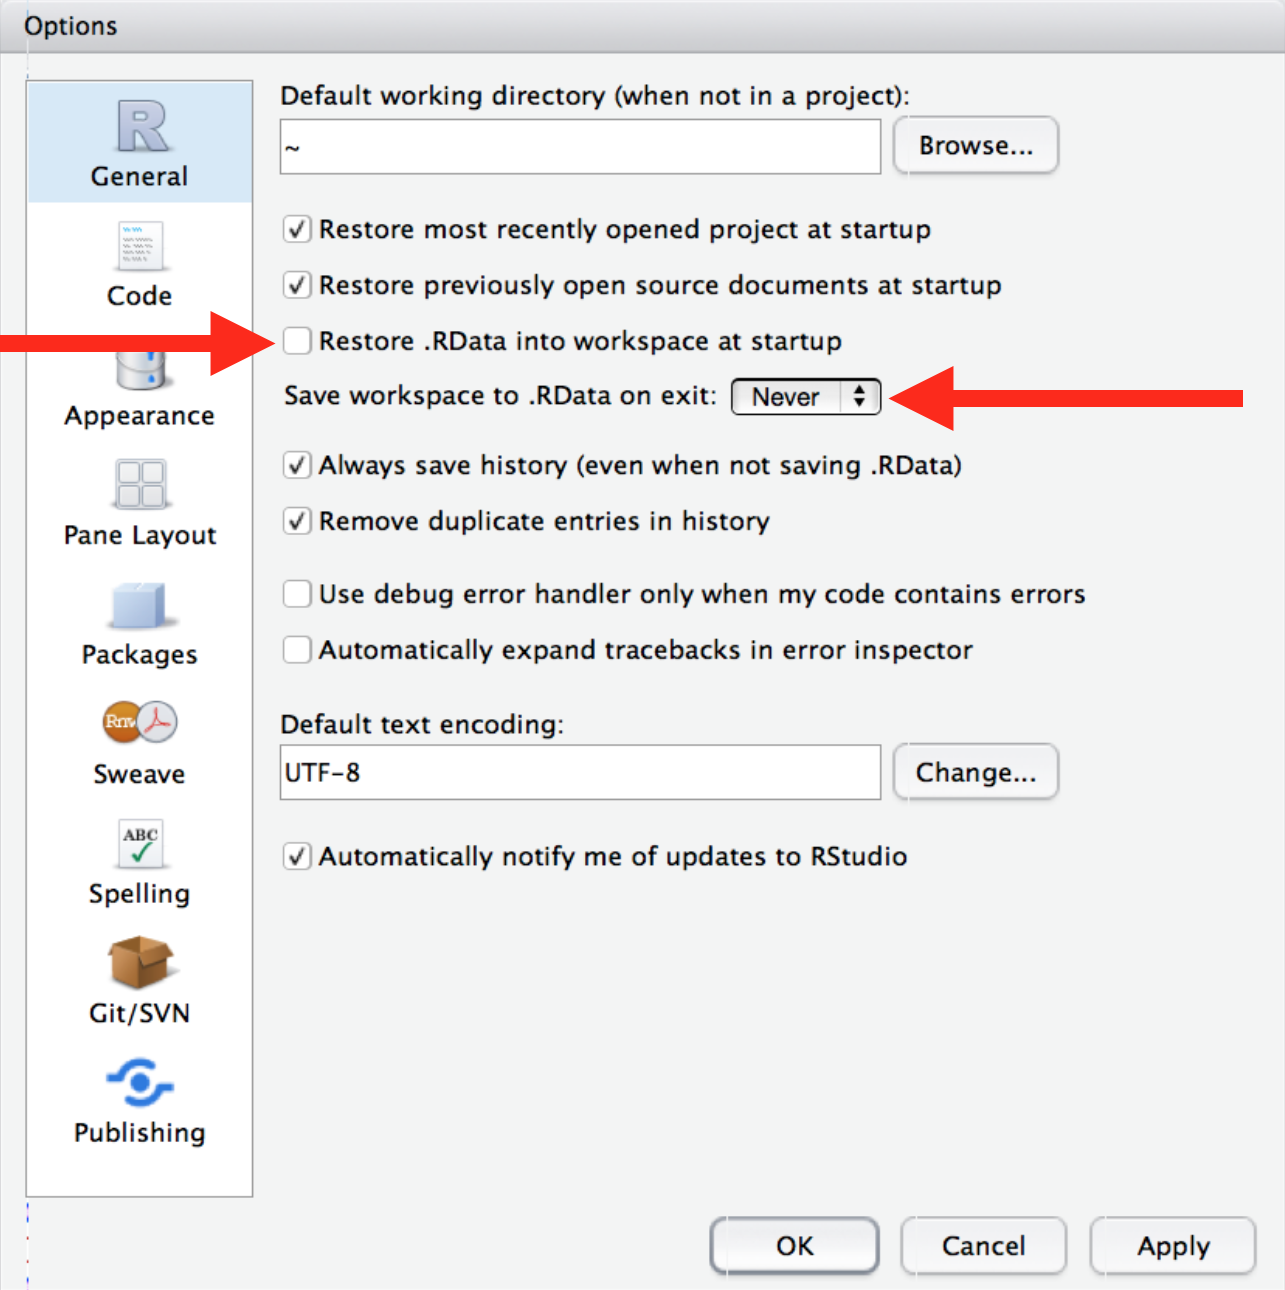
\includegraphics[width=0.75\linewidth]{screenshots/rstudio-workspace} \end{center}

This will cause you some short-term pain, because now when you restart
RStudio it will not remember the results of the code that you ran last
time. But this short-term pain will save you long-term agony because it
forces you to capture all important interactions in your code. There's
nothing worse than discovering three months after the fact that you've
only stored the results of an important calculation in your workspace,
not the calculation itself in your code.

There is a great pair of keyboard shortcuts that will work together to
make sure you've captured the important parts of your code in the
editor:

\begin{enumerate}
\def\labelenumi{\arabic{enumi}.}
\tightlist
\item
  Press Cmd/Ctrl + Shift + F10 to restart RStudio.
\item
  Press Cmd/Ctrl + Shift + S to rerun the current script.
\end{enumerate}

I use this pattern hundreds of times a week.

\newpage

\hypertarget{where-does-your-analysis-live}{%
\section{Where does your analysis
live?}\label{where-does-your-analysis-live}}

R has a powerful notion of the \textbf{working directory}. This is where
R looks for files that you ask it to load, and where it will put any
files that you ask it to save. RStudio shows your current working
directory at the top of the console:

\begin{center}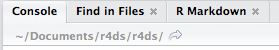
\includegraphics[width=0.5\linewidth]{screenshots/rstudio-wd} \end{center}

And you can print this out in R code by running \texttt{getwd()}:

\begin{Shaded}
\begin{Highlighting}[]
\KeywordTok{getwd}\NormalTok{()}
\CommentTok{#> [1] "/Users/hadley/Documents/r4ds/r4ds"}
\end{Highlighting}
\end{Shaded}

As a beginning R user, it's OK to let your home directory, documents
directory, or any other weird directory on your computer be R's working
directory. But you're six chapters into this book, and you're no longer
a rank beginner. Very soon now you should evolve to organising your
analytical projects into directories and, when working on a project,
setting R's working directory to the associated directory.

\textbf{I do not recommend it}, but you can also set the working
directory from within R:

\begin{Shaded}
\begin{Highlighting}[]
\KeywordTok{setwd}\NormalTok{(}\StringTok{"/path/to/my/CoolProject"}\NormalTok{)}
\end{Highlighting}
\end{Shaded}

But you should never do this because there's a better way; a way that
also puts you on the path to managing your R work like an expert.

\hypertarget{paths-and-directories}{%
\section{Paths and directories}\label{paths-and-directories}}

Paths and directories are a little complicated because there are two
basic styles of paths: Mac/Linux and Windows. There are three chief ways
in which they differ:

\begin{enumerate}
\def\labelenumi{\arabic{enumi}.}
\item
  The most important difference is how you separate the components of
  the path. Mac and Linux uses slashes
  (e.g.~\texttt{plots/diamonds.pdf}) and Windows uses backslashes
  (e.g.~\texttt{plots\textbackslash{}diamonds.pdf}). R can work with
  either type (no matter what platform you're currently using), but
  unfortunately, backslashes mean something special to R, and to get a
  single backslash in the path, you need to type two backslashes! That
  makes life frustrating, so I recommend always using the Linux/Mac
  style with forward slashes.
\item
  Absolute paths (i.e.~paths that point to the same place regardless of
  your working directory) look different. In Windows they start with a
  drive letter (e.g.~\texttt{C:}) or two backslashes
  (e.g.~\texttt{\textbackslash{}\textbackslash{}servername}) and in
  Mac/Linux they start with a slash ``/'' (e.g.~\texttt{/users/hadley}).
  You should \textbf{never} use absolute paths in your scripts, because
  they hinder sharing: no one else will have exactly the same directory
  configuration as you.
\item
  The last minor difference is the place that \texttt{\textasciitilde{}}
  points to. \texttt{\textasciitilde{}} is a convenient shortcut to your
  home directory. Windows doesn't really have the notion of a home
  directory, so it instead points to your documents directory.
\end{enumerate}

\hypertarget{rstudio-projects}{%
\section{RStudio projects}\label{rstudio-projects}}

R experts keep all the files associated with a project together ---
input data, R scripts, analytical results, figures. This is such a wise
and common practice that RStudio has built-in support for this via
\textbf{projects}.

Let's make a project for you to use while you're working through the
rest of this book. Click File \textgreater{} New Project, then:

\begin{center}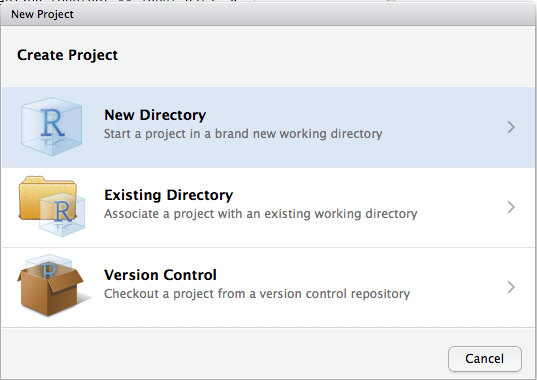
\includegraphics[width=0.5\linewidth]{screenshots/rstudio-project-1} \end{center}

\begin{center}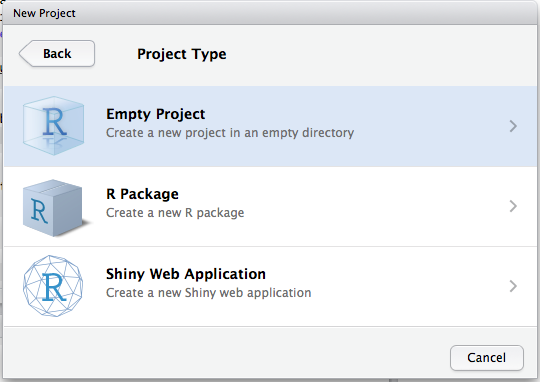
\includegraphics[width=0.5\linewidth]{screenshots/rstudio-project-2} \end{center}

\begin{center}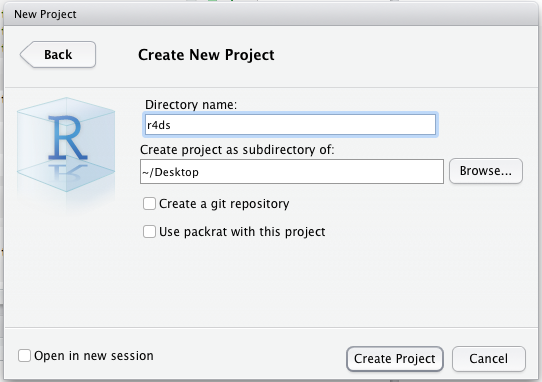
\includegraphics[width=0.5\linewidth]{screenshots/rstudio-project-3} \end{center}

Call your project \texttt{r4ds} and think carefully about which
\emph{subdirectory} you put the project in. If you don't store it
somewhere sensible, it will be hard to find it in the future!

Once this process is complete, you'll get a new RStudio project just for
this book. Check that the ``home'' directory of your project is the
current working directory:

\begin{Shaded}
\begin{Highlighting}[]
\KeywordTok{getwd}\NormalTok{()}
\CommentTok{#> [1] /Users/hadley/Documents/r4ds/r4ds}
\end{Highlighting}
\end{Shaded}

Whenever you refer to a file with a relative path it will look for it
here.

Now enter the following commands in the script editor, and save the
file, calling it ``diamonds.R''. Next, run the complete script which
will save a PDF and CSV file into your project directory. Don't worry
about the details, you'll learn them later in the book.

\begin{Shaded}
\begin{Highlighting}[]
\KeywordTok{library}\NormalTok{(tidyverse)}

\KeywordTok{ggplot}\NormalTok{(diamonds, }\KeywordTok{aes}\NormalTok{(carat, price)) }\OperatorTok{+}\StringTok{ }
\StringTok{  }\KeywordTok{geom_hex}\NormalTok{()}
\KeywordTok{ggsave}\NormalTok{(}\StringTok{"diamonds.pdf"}\NormalTok{)}

\KeywordTok{write_csv}\NormalTok{(diamonds, }\StringTok{"diamonds.csv"}\NormalTok{)}
\end{Highlighting}
\end{Shaded}

Quit RStudio. Inspect the folder associated with your project --- notice
the \texttt{.Rproj} file. Double-click that file to re-open the project.
Notice you get back to where you left off: it's the same working
directory and command history, and all the files you were working on are
still open. Because you followed my instructions above, you will,
however, have a completely fresh environment, guaranteeing that you're
starting with a clean slate.

In your favorite OS-specific way, search your computer for
\texttt{diamonds.pdf} and you will find the PDF (no surprise) but
\emph{also the script that created it} (\texttt{diamonds.R}). This is
huge win! One day you will want to remake a figure or just understand
where it came from. If you rigorously save figures to files \textbf{with
R code} and never with the mouse or the clipboard, you will be able to
reproduce old work with ease!

\hypertarget{summary}{%
\section{Summary}\label{summary}}

In summary, RStudio projects give you a solid workflow that will serve
you well in the future:

\begin{itemize}
\item
  Create an RStudio project for each data analysis project.
\item
  Keep data files there; we'll talk about loading them into R in {[}data
  import{]}.
\item
  Keep scripts there; edit them, run them in bits or as a whole.
\item
  Save your outputs (plots and cleaned data) there.
\item
  Only ever use relative paths, not absolute paths.
\end{itemize}

Everything you need is in one place, and cleanly separated from all the
other projects that you are working on.

%\showmatmethods





\end{document}

